%%%%%%%%%%%%%%%%%%%%%%%%%%%%%%%%%%%%%%%%%%%%%%%%%%%%%%%%%%%%%%%%%%%%%%%%%%%%%%%
% Chapter 4 - Improving Cerebral Blood Flow Measurements with Multi-Exposure Speckle Imaging
%%%%%%%%%%%%%%%%%%%%%%%%%%%%%%%%%%%%%%%%%%%%%%%%%%%%%%%%%%%%%%%%%%%%%%%%%%%%%%%

\chapter{Improving Cerebral Blood Flow Measurements with Multi-Exposure Speckle Imaging} \label{ch:mesi}

While the conventional LSCI technique can provide reliable measurements of relative flow, it is incapable of quantifying absolute baseline values. This complicates the chronic study and inter-animal comparisons of blood flow dynamics because variations in imaging conditions cannot be properly accounted for by the underlying model. This has not prevented LSCI from being used to study chronic changes in flow (see Section \ref{sec:chronic_hemodynamics}), but has limited the observations to predominantly qualitative interpretations \cite{Armitage:2010ga}. The technique has also been shown to underestimate large changes in flow and fails to produce reliable measurements in the presence of static scatters \cite{Parthasarathy:2008el}.

Multi-exposure speckle imaging (MESI) is an extension to traditional LSCI theory that accounts for static scattering and produces a more robust estimate of $\tau_c$ using multiple camera exposure times \cite{Parthasarathy:2008el}. These improvements are achieved by accounting for the heterodyne mixing of dynamic and static scattering contributions, the non-ergodicity of light, and exposure-independent noise. The model described by Parthasarathy \textit{et al.} \cite{Parthasarathy:2008el} again relates the measured $K$ with $\tau_c$:

% Equation - MESI Equation
\begin{equation}
    \label{eq:mesi}
    \resizebox{\textwidth}{!}{$
    K(T,\tau_c) =
        \left(
        \beta\rho^2\frac{e^{-2x} - 1 + 2x}{2x^2} +
        4\beta\rho(1 - \rho)\frac{e^{-x} - 1 + x}{x^2} +
        \beta(1 - \rho)^2 +
        \nu_{ne} +
        \nu_{noise}
        \right)^{1/2}
    $}
\end{equation}

\noindent where $x = T/\tau_c$, $T$ is the camera exposure time, $\beta$ is the same normalization factor that accounts for speckle averaging effects, $\rho$ is the fraction of light that is dynamically scattered, $\nu_{ne}$ is the constant variance due to nonergodic light, and $\nu_{noise}$ is the exposure-independent instrument noise. For simplicity, $\nu_{ne}$ and $\nu_{noise}$ are typically merged into a single noise parameter ($\nu_{noise}$). Similar to Equation \ref{eq:bandyopadhyay}, this expression assumes that detected photons only experience single scattering interactions and that the underlying particle motion has a Lorentzian velocity distribution. A scaling term representing the number of average dynamic scattering events can be included with $x$ to account for multiple scattering interactions \cite{Kazmi:2015du}. In the absence of static scatterers, $\rho \to 1$ and Equation \ref{eq:mesi} simplifies to Equation \ref{eq:bandyopadhyay}, excluding the noise terms. In the presence of only static scatterers, then $\rho \to 0$ and $K$ reduces to a constant $\beta(1 - \rho)^2 + \nu_{noise}$ and is independent of exposure time. This represents the upper limit of the speckle variance ($K^2$) as $T$ approaches infinity. The lower limit as $T$ approaches 0 is $\beta + \nu_{noise}$, which can be approximated with just $\beta$ because the noise will only constitute a small percentage of the total value.

A minimum of four speckle contrast images acquired at different exposure times are necessary to fit Equation \ref{eq:mesi} for the four unknown variables ($\beta$, $\rho$, $\tau_c$, $\nu_{noise}$). In practice, 15 images spanning three decades of exposure times (50 $\mu$s - 80 ms) are typically utilized to sample as much of the underlying flow distribution as possible. The MESI model has improved the quantitative accuracy of flow measurements in controlled microfluidic environments \cite{Parthasarathy:2008el, Kazmi:2015du} and closely approximates the results of direct autocorrelation measurements \cite{Kazmi:2015ji}. The technique has enabled the chronic study of CBF across multiple animals and improved the robustness of flow deficit measurements during stroke \cite{Parthasarathy:2010vo, Kazmi:2013hp, Schrandt:2015gu}. This chapter details an upgrade to the imaging system to perform MESI and further validation of its capabilities.



%%%%%%%%%%%%%%%%%%%%%%%%%%%%%%%%%%%%%%%%%%%%%%%%%%%%%%%%%%%%%%%%%%%%%%%%%%%%%%%
% Section 4.1 - Instrumentation Modifications
%%%%%%%%%%%%%%%%%%%%%%%%%%%%%%%%%%%%%%%%%%%%%%%%%%%%%%%%%%%%%%%%%%%%%%%%%%%%%%%
\section{Instrumentation Modifications}

The instrumentation necessary for performing MESI is similar to traditional LSCI but requires precise control over both the camera exposure time and the laser intensity. Varying the exposure time alone would result in shot noise overwhelming the speckle signal at longer exposure times because of differences in intensity. However, by modulating the amplitude of the illuminating laser light, the average intensity of the images, and therefore the shot noise, can be held constant. Passive optical devices such as AOMs have historically been used to avoid the bandwidth and dynamic range limitations of direct laser diode modulation.

Figure \ref{fig:systemschematic_3} depicts the modifications made to the LSCI illumination pathway in order to perform MESI with the system. The same 685 nm laser diode (50 mW, HL6750MG, Thorlabs, Inc.) was collimated using an aspheric lens (C240TME-B, Thorlabs, Inc.) and the beam diameter was reduced to 1 mm. The light was modulated using a 100 MHz AOM (3100-125 AOM + 1110AF-AIFO-1.0 RF Driver, Gooch \& Housego) with the first order diffraction isolated and relayed to obliquely illuminate the sample. The camera was also upgraded (acA1920-155um, 1920 x 1200 pixels, Basler AG) because the previous model did not support trigger-based control of exposure duration, which is important for implementing MESI. The new camera also offered more convenient USB 3.0 connectivity, higher maximum frame rate (164 fps), lower dark noise, and increased dynamic range. While the pixel resolution was almost doubled, only a subset of the overall sensor array was used (1200 x 1200 pixels), resulting in a FOV of 3.6 x 3.6 mm.

% Figure - System Schematic (Ver. 3)
\begin{figure}
    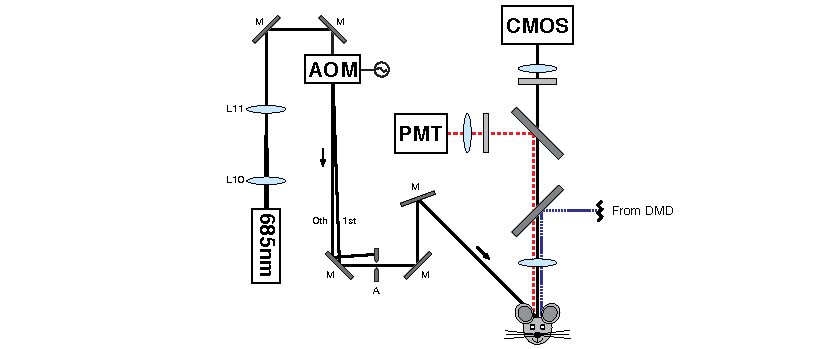
\includegraphics{figures/chapter_4/systemschematic_3.pdf}
    \caption{
        \label{fig:systemschematic_3}
        The optical system was modified to perform MESI with the addition of an AOM to modulate the 685 nm laser used for LSCI.
    }
\end{figure}

%%%%%%%%%%%%%%%%%%%%%%%%%%%%%%%%%%%%%%%%%%%%%%%%%%%%%%%%%%%%%%%%%%%%%%%%%%%%%%%
\subsection{Acquisition Control}

The MESI acquisition process is controlled by a combination of the Speckle Software and a standalone MATLAB (MathWorks, Inc.) script. The software was updated to allow the camera to perform "Trigger Width Exposure Mode" acquisitions, where the duration of a hardware trigger signal directly controls the exposure time of each frame. The MATLAB script used the ANSI C NI-DAQmx library (National Instruments Corp.) to operate a multifunction I/O device (USB-6363, National Instruments Corp.) to produce the camera exposure trigger signals and AOM modulation voltages (Figure \ref{fig:mesitimingschematic}). Both waveforms were generated at 1 MHz with identical pulse durations but a slight temporal offset (+25 $\mu$s delay for the AOM signal) to guarantee that the actual camera exposures and the laser pulses were synchronized in time. This was validated using the “Exposure Active” output signal from the camera and a photodiode (PDA36A, Thorlabs, Inc.) directly measuring the modulated laser.

A complete MESI frame consists of 15 raw intensity images (8-bit) each acquired with a different exposure time for an effective frame rate of 2.5 fps without any averaging. This is significantly slower than standard LSCI and insufficient to properly sample faster hemodynamic processes. Because of limitations with the Speckle Software, the speckle contrast images cannot be computed for real-time visualization during an acquisition. This requires the speckle contrast images to be generated during post-processing. A standard MESI acquisition produces data at a rate of 178 MB/s.

% Figure - MESI Timing
\begin{figure}
    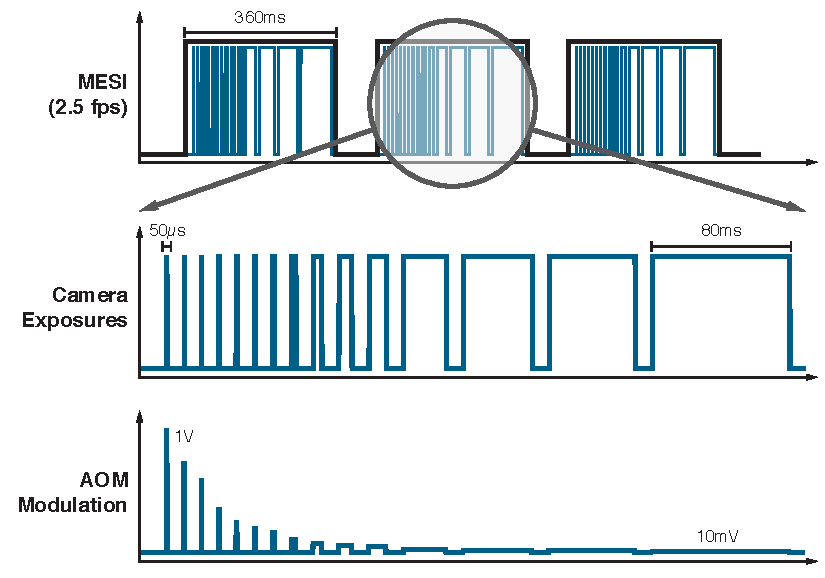
\includegraphics{figures/chapter_4/mesitimingschematic.pdf}
    \caption{
        \label{fig:mesitimingschematic}
        Timing paradigm for MESI camera exposure triggers and AOM modulation voltages. The integration of each AOM pulse over time is equal.
    }
\end{figure}

%%%%%%%%%%%%%%%%%%%%%%%%%%%%%%%%%%%%%%%%%%%%%%%%%%%%%%%%%%%%%%%%%%%%%%%%%%%%%%%
\subsection{Calibration Procedure}

The AOM modulation voltages for each exposure are determined using the calibration procedure outlined in Figure \ref{fig:mesicalibration}. This process ensures that shot noise is held constant across all exposures by equalizing the total amount of light used to produce each image. Because the reflectivity of the imaging surface varies by sample, the calibration must be performed prior to each MESI experiment.

% Figure - MESI Calibration
\begin{figure}
    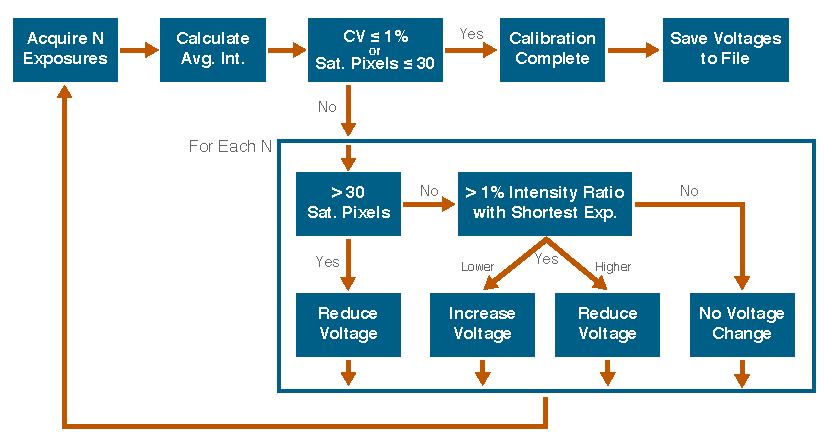
\includegraphics{figures/chapter_4/mesicalibration.pdf}
    \caption{
        \label{fig:mesicalibration}
        Overview of the MESI calibration process that attempts to equalize the raw image intensities while minimizing saturated pixels across all $N$ exposures.
    }
\end{figure}

The initial guess for the modulation voltages is generated using a power law function confined between 0-1 V. These voltages are used to acquire a complete MESI frame containing 15 raw intensity images from different exposures. The average intensity and total number of saturated pixels within a user-defined region is then calculated for each image. If the overall coefficient of variation and the number of saturated pixels are less than the defined thresholds, then the intensities are equalized and the calibration is complete. However, if the average intensity variation is too high or if there are too many saturated pixels, then each of the modulation voltages are adjusted accordingly using the shortest exposure time as the target intensity. This process repeats recursively until the stop conditions are achieved.

Figure \ref{fig:rawmesi} contains an example of the final iteration of a MESI calibration for an \textit{in vivo} imaging experiment. The intensity-equalized raw images for each of the 15 exposures can be seen in Figure \ref{fig:rawmesi}A. The speckle pattern becomes increasingly blurred, especially within vascular regions, as the camera integration time increases. The average intensity from the center quadrant of each exposure is shown in Figure \ref{fig:rawmesi}B, with a final coefficient of variation \textless1\%. Figure \ref{fig:rawmesi}C depicts the resulting calibrated AOM modulation voltages for use with each exposure time during the actual imaging experiment. The voltages span two orders of magnitude (0.3 V - 3 mV) and cover the entire modulation range of the AOM.

% Figure - MESI Raw
\begin{figure}
    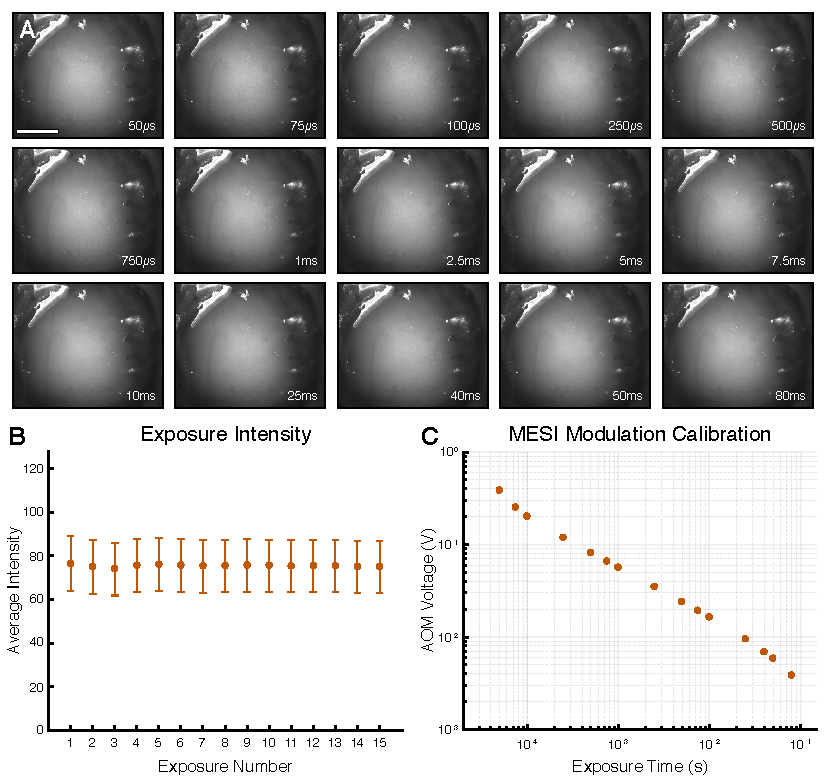
\includegraphics{figures/chapter_4/rawmesi.pdf}
    \caption{
        \label{fig:rawmesi}
        \textbf{(A)} Raw images of a cranial window from each of the 15 MESI exposures acquired using calibrated modulation voltages to equalize intensity (Scale bar = 1 mm). \textbf{(B)} Average intensity from the center quadrant of each image (mean $\pm$ s.d.). \textbf{(C)} Calibrated MESI modulation voltages for each exposure time.
    }
\end{figure}



%%%%%%%%%%%%%%%%%%%%%%%%%%%%%%%%%%%%%%%%%%%%%%%%%%%%%%%%%%%%%%%%%%%%%%%%%%%%%%%
% Section 4.2 - Improving MESI Processing Speed
%%%%%%%%%%%%%%%%%%%%%%%%%%%%%%%%%%%%%%%%%%%%%%%%%%%%%%%%%%%%%%%%%%%%%%%%%%%%%%%
\section{Improving MESI Processing Speed}

\blindtext



%%%%%%%%%%%%%%%%%%%%%%%%%%%%%%%%%%%%%%%%%%%%%%%%%%%%%%%%%%%%%%%%%%%%%%%%%%%%%%%
% Section 4.3 - Demonstration of In Vivo MESI
%%%%%%%%%%%%%%%%%%%%%%%%%%%%%%%%%%%%%%%%%%%%%%%%%%%%%%%%%%%%%%%%%%%%%%%%%%%%%%%
\section{Demonstration of \textit{In Vivo} MESI}

\blindtext



%%%%%%%%%%%%%%%%%%%%%%%%%%%%%%%%%%%%%%%%%%%%%%%%%%%%%%%%%%%%%%%%%%%%%%%%%%%%%%%
% Section 4.4 - Reproducibility and Stability of MESI
%%%%%%%%%%%%%%%%%%%%%%%%%%%%%%%%%%%%%%%%%%%%%%%%%%%%%%%%%%%%%%%%%%%%%%%%%%%%%%%
\section{Reproducibility and Stability of MESI}

\blindtext



%%%%%%%%%%%%%%%%%%%%%%%%%%%%%%%%%%%%%%%%%%%%%%%%%%%%%%%%%%%%%%%%%%%%%%%%%%%%%%%
% Section 4.5 - Discussion
%%%%%%%%%%%%%%%%%%%%%%%%%%%%%%%%%%%%%%%%%%%%%%%%%%%%%%%%%%%%%%%%%%%%%%%%%%%%%%%
\section{Discussion}

\blindtext



%%%%%%%%%%%%%%%%%%%%%%%%%%%%%%%%%%%%%%%%%%%%%%%%%%%%%%%%%%%%%%%%%%%%%%%%%%%%%%%
% END Chapter 4
%%%%%%%%%%%%%%%%%%%%%%%%%%%%%%%%%%%%%%%%%%%%%%%%%%%%%%%%%%%%%%%%%%%%%%%%%%%%%%%
